
%%%%%%%%%%%%%%%%%%%%%%%%%%%%%%%%%%%%%%%%%%%%%%%%%%%%%%%%%%%%%%%%%%%%%%%%%%%%%%%
% PREAMBLE %%%%%%%%%%%%%%%%%%%%%%%%%%%%%%%%%%%%%%%%%%%%%%%%%%%%%%%%%%%%%%%%%%%%
%%%%%%%%%%%%%%%%%%%%%%%%%%%%%%%%%%%%%%%%%%%%%%%%%%%%%%%%%%%%%%%%%%%%%%%%%%%%%%%

\documentclass[
    10pt,
    conference,
    % draftcls,
    % draftclsnofoot,
    compsocconf
]{IEEEtran}

\usepackage[pdftex]{graphicx}
\graphicspath{{../images/}}
\DeclareGraphicsExtensions{.pdf,.jpeg,.png}
%\usepackage[cmex10]{amsmath}
%\usepackage{algorithmic}
%\usepackage{array}
%\usepackage{mdwmath}
%\usepackage{mdwtab}
%\usepackage{eqparbox}
\usepackage[tight,footnotesize]{subfigure}
\usepackage[caption=false,font=footnotesize]{subfig}
\newcounter{subfigure@save}
\usepackage{url}

% correct bad hyphenation here
\hyphenation{op-tical net-works semi-conduc-tor}

%%%%%%%%%%%%%%%%%%%%%%%%%%%%%%%%%%%%%%%%%%%%%%%%%%%%%%%%%%%%%%%%%%%%%%%%%%%%%%%
% TITLE %%%%%%%%%%%%%%%%%%%%%%%%%%%%%%%%%%%%%%%%%%%%%%%%%%%%%%%%%%%%%%%%%%%%%%%
%%%%%%%%%%%%%%%%%%%%%%%%%%%%%%%%%%%%%%%%%%%%%%%%%%%%%%%%%%%%%%%%%%%%%%%%%%%%%%%

\begin{document}
\title{TorusVis: A Topology Data Visualization Tool}
\author{
    \IEEEauthorblockN{Omar Padron, Dave Semeraro}
    \IEEEauthorblockA{
        National Center for Supercomputing Applications \\
        University of Illinois at Urbana Champaign      \\
        Urbana, IL USA                                  \\
        \{opadron, semeraro\}@illinois.edu
    }
}

% \IEEEspecialpapernotice{(DRAFT IN PREPARATION)}

\maketitle

%%%%%%%%%%%%%%%%%%%%%%%%%%%%%%%%%%%%%%%%%%%%%%%%%%%%%%%%%%%%%%%%%%%%%%%%%%%%%%%
% ABSTRACT %%%%%%%%%%%%%%%%%%%%%%%%%%%%%%%%%%%%%%%%%%%%%%%%%%%%%%%%%%%%%%%%%%%%
%%%%%%%%%%%%%%%%%%%%%%%%%%%%%%%%%%%%%%%%%%%%%%%%%%%%%%%%%%%%%%%%%%%%%%%%%%%%%%%

\begin{abstract}
    The ever-growing scope of extreme-scale supercomputers requires an
    increasing volume of component-local metrics to better understand their
    systemic behavior.  The collection and analysis of these metrics have
    become data-intensive tasks in their own right, the products of which inform
    system support activities critical to ongoing operations.  With recent
    emphasis being placed on topology-awareness as a step towards better coping
    with extreme scale, the ability to visualize complex topology data has
    become increasingly valuable, particularly for the visualization of
    multidimensional tori.  Several independent efforts to produce similar
    visualizations exist, but they have typically been in-house developments
    tailor-made for very specific purposes; and not trivially applicable to
    visualization needs not featured among those purposes.  In contrast, a more
    general-purpose tool offers benefits that ease understanding of many
    interrelated aspects of a system's behavior, such as application
    performance, job node placement, and network traffic patterns.  Perhaps more
    significantly, such a tool can offer analysts insight into the complex
    topological relationships shared among these considerations; relationships
    that are often difficult to quantify by any other means.

    We present TorusVis, a general-purpose visualization tool applicable to a
    wide variety of topology-related data presentation scenarios.  Its
    general-purpose software architecture lends itself well to rapid prototyping
    of various data presentation concepts as well as publishing fully featured
    visualizations.  We describe several key design elements and implementation
    strategies, and how they strike a balance between usability, generality, and
    simplicity.  Furthermore, we present use case studies where the capabilities
    available in TorusVis aided understanding of system behavior in ways not
    possible, otherwise.
\end{abstract}

\begin{IEEEkeywords}
    visualization; performance analysis; system monitoring
\end{IEEEkeywords}

\IEEEpeerreviewmaketitle

%%%%%%%%%%%%%%%%%%%%%%%%%%%%%%%%%%%%%%%%%%%%%%%%%%%%%%%%%%%%%%%%%%%%%%%%%%%%%%%
% INTRODUCTION %%%%%%%%%%%%%%%%%%%%%%%%%%%%%%%%%%%%%%%%%%%%%%%%%%%%%%%%%%%%%%%%
%%%%%%%%%%%%%%%%%%%%%%%%%%%%%%%%%%%%%%%%%%%%%%%%%%%%%%%%%%%%%%%%%%%%%%%%%%%%%%%

\section{Introduction}
% no \IEEEPARstart
    System monitoring is an absolutely vital task for effectively operating HPC
    resources.  Whether they are support staff helping users optimize their
    applications, maintenance personnel detecting and resolving issues, or
    administrators reconfiguring system behavior, detailed system metrics
    empower both operators and users to maximize the productive value of their
    computing resources.  As the capabilities of modern systems are pushed
    further towards exascale, so too are the complexities involved with the
    collection, analysis, and representation of operational metrics data.

    For example, the placement of applications on a system's compute network can
    give clues about application performance.  Information about which nodes are
    used by an application, the placement of those nodes on the communication
    fabric, the relative location of other applications, and the relative
    location of service nodes can be used to better characterize application
    performance and provide insight on the modifications best suited for
    maximizing it.  Application placement and performance data can be further
    augmented with system data (e.g. from event logs) and better guide
    diagnostic efforts.

    All of this information is readily available on most HPC systems, but
    in addition to the growing costs of collecting, storing, and curating it;
    HPC support staff are faced with the challenge of representing analysis
    results in a form accessible by human comprehension.  One natural choice is
    an interactive 3D visualization where the system topology is represented by
    a graph mesh whose visual characteristics, such as node color, size, and
    shape, are modulated to convey the operational data of interest to an
    analyst.

    In this paper, we discuss the topology data visualization work performed at
    NCSA in support of the Blue Waters project.  We present several realized
    usage scenarios and discuss how our early software prototypes empowered
    operations staff to better understand system behavior and application
    performance.  We also discuss some hypothetical capabilities for other
    anticipated use cases, and their potential value to the HPC community.  This
    potential motivates our recent efforts to channel the development
    experiences gained into a new modular and general-purpose topology data
    visualization software library we have named ``TorusVis''.  We briefly
    outline the core software design of TorusVis, and conclude with our future
    plans, which include releasing it for the community under an open-source
    license.

%%%%%%%%%%%%%%%%%%%%%%%%%%%%%%%%%%%%%%%%%%%%%%%%%%%%%%%%%%%%%%%%%%%%%%%%%%%%%%%
% CASE STUDIES %%%%%%%%%%%%%%%%%%%%%%%%%%%%%%%%%%%%%%%%%%%%%%%%%%%%%%%%%%%%%%%%
%%%%%%%%%%%%%%%%%%%%%%%%%%%%%%%%%%%%%%%%%%%%%%%%%%%%%%%%%%%%%%%%%%%%%%%%%%%%%%%

\section{Case Studies}
 
    \begin{figure*}[!t]
        \centering
        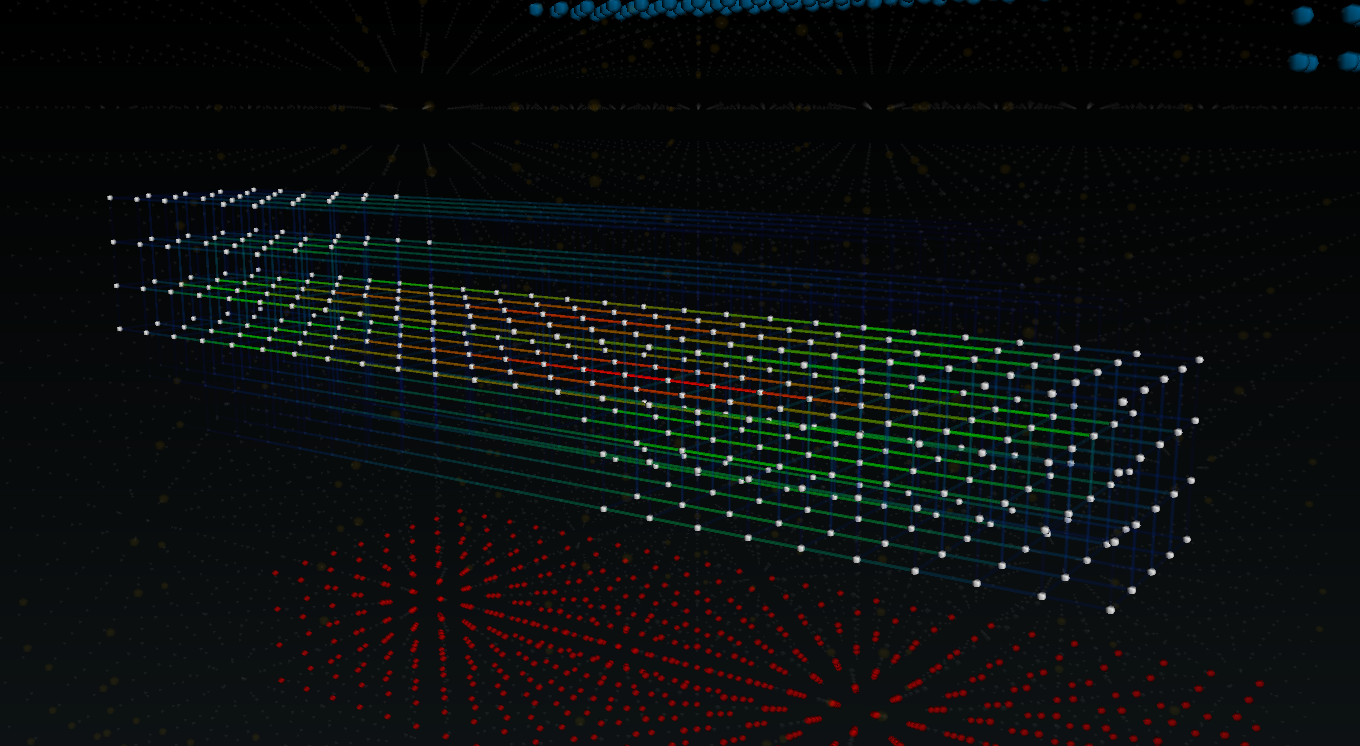
\includegraphics[width=6.5in]{215389-all-to-all}
        \caption{
            Visualization of an irregularly-shaped job node placement.  The
            links among the various nodes are mapped to color and transparency
            values based on a heuristic model that estimates the relative
            congestion for an all-to-all communication pattern.  This rendering
            demonstrates a priori analysis capabilities made possible by
            topology visualization tools.
        }
        \label{fig_all2all}
    \end{figure*}
  
    The display of the placement of user jobs and system resources in relation
    to the communication topology has a number of uses. For example, job
    performance may be impacted by the location of the job nodes in relation to
    each other and system resources. A variety of information can be displayed
    in addition to just node placement. Network traffic, for example, is an
    important metric that, if visualized over time on the network can reveal
    patterns that may aid the analyst in improving application performance. An
    example of this capability is illustrated in Figure \ref{fig_all2all}.

    \begin{figure}[!t]
        \centering
        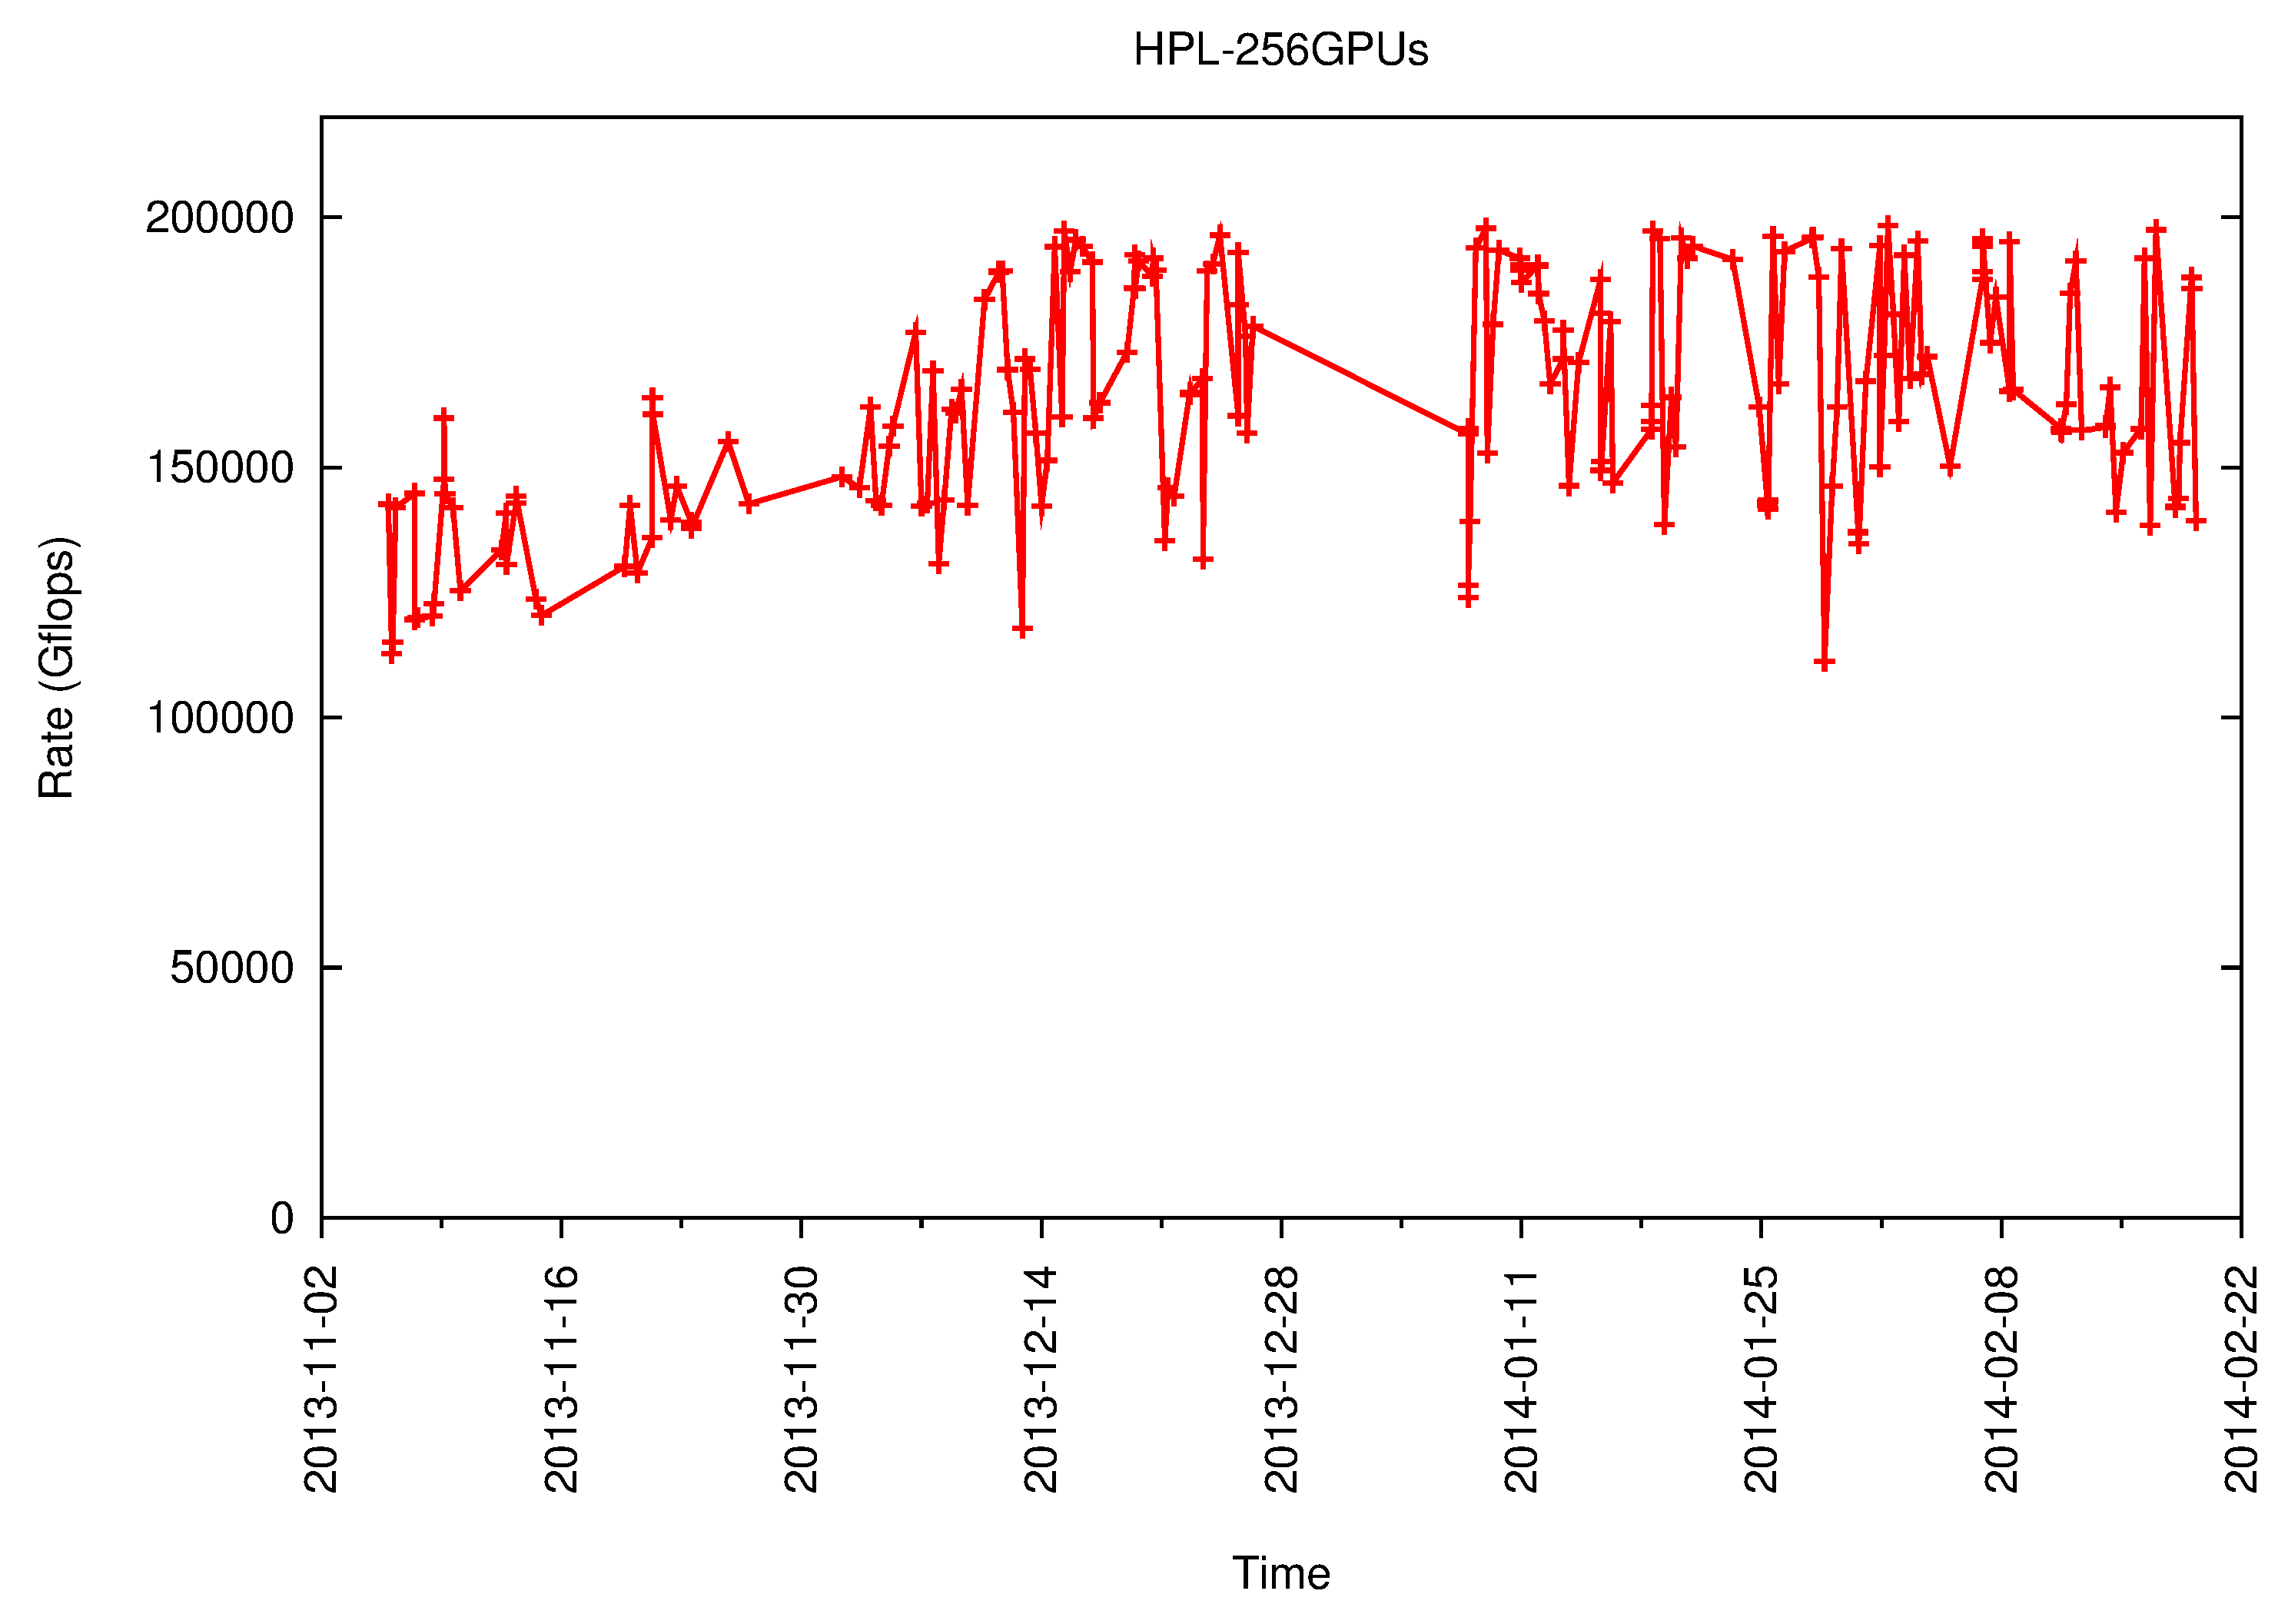
\includegraphics[width=3.5in]{celso-hpl-bw}
        \caption{
            Application performance (in GFLOPS) for several 256-node runs of a
            GPU-enabled version of HPL performed over a period of about three
            months.  Performance varies by almost a factor of two in the
            best-to-worst case comparison, despite there being no changes in job
            configuration.
        }
        \label{hpl_plot}
    \end{figure}

    Our early work on visualization application prototypes was primarily
    motivated by a series of studies performed with partners from Cray and
    Adaptive Computing on the run time consistency of applications ran on the
    Blue Waters system.  We observed that many applications required highly
    variable amounts of compute time for seemingly identical runs.  We began to
    investigate system factors that might contribute to this variability, and
    identified job node placement as a factor that was likely to affect job run
    time.  We hypothesized that jobs with node placements that were more compact
    would perform better than those with placements more spread throughout the
    torus.  We proposed several metrics in an attempt to quantify the
    compactness of these placements, such as maximum, average, or a profile of
    hop counts among node pairs.  However, we found that the correlation between
    each of our tested metrics and job run time were weak, and that they were
    poor performance predictors.  We considered other likely factors, such as
    interfering traffic from other jobs, or external system events, and realized
    that job run time was likely a non-trivial function of all of these
    considerations.  We turned to visualization as a way to observe the data
    collected on each of these aspects and identify trends intuitively.

    \begin{figure*}[!t]
        \centerline{
            \subfloat{%[Worst HPL Run] {
                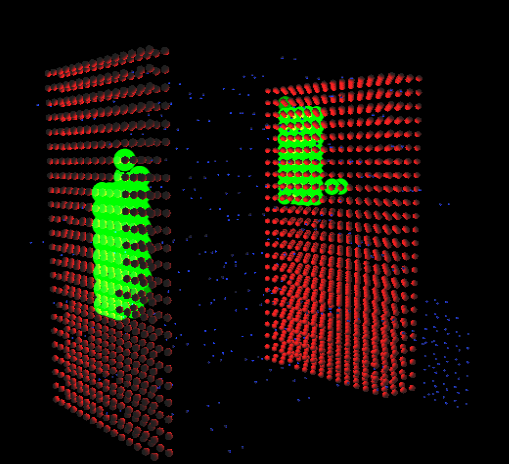
\includegraphics[width=3.0in]{celso-567784}
                \label{hpl_slow}
            }
            \hfil
            \subfloat{%[Best HPL Run] {
                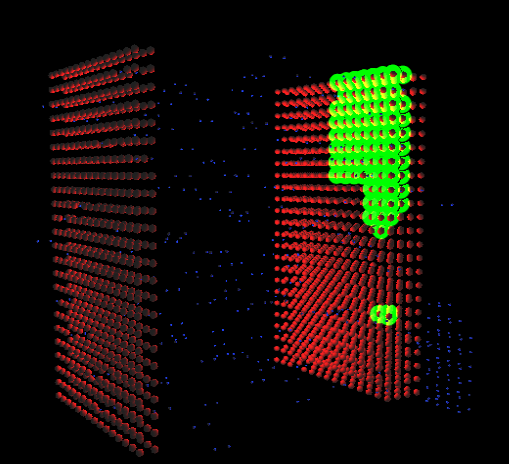
\includegraphics[width=3.0in]{celso-595916}
                \label{hpl_fast}
            }
        }

        \caption{
            Visualization of the node placements for the best, and worse
            performing HPL runs.  The worse performing run used a node
            allocation of two distinct, segregated regions (\emph{left}), while
            the best performing run used one that was clearly more compact
            (\emph{right}).
        }
        \label{hpl_slow_fast}
    \end{figure*}


    We found that job node placement did, indeed, have a major impact on run
    time, but often in ways that were not simple to quantify.  Figure
    \ref{hpl_plot} shows application performance for several runs of HPL that
    were identical except for the placement of their job's nodes.  The best
    performing job achieved a performance of 197.5 TFLOPS and outperformed the
    111.2 TFLOPS performance of the worst performing job by nearly a factor of
    two.  Figure \ref{hpl_slow_fast} shows the node placements for both cases.
    The visualizations show that the worst performing job used a node allocation
    of two distinct, segregated regions; most likely resulting in high
    communication overhead.  Although the best performing job used an allocation
    that, in an apparent, albeit qualitative sense, was more compact, it too had
    a few outlying nodes.  The latter allocation was clearly superior to the
    former, though to an extent not well represented through purely quantitative
    analysis.

    Another use for topology visualization is for showing the system resources
    on the torus.  This is particularly useful when warm swapping components in
    and out of the system.  Maintenance staff must exercise extreme caution when
    servicing the system to ensure that the correct components are pulled out.
    Accidentally removing operational hardware may cause holes in the torus
    network that could result in unroutable conditions.  System components must
    be warm swapped very carefully to avoid adversely impacting running
    applications.  Our topology visualization applications aid maintenance staff
    in verifying the location of target components.

\begin{figure}[!t]
	\centering
	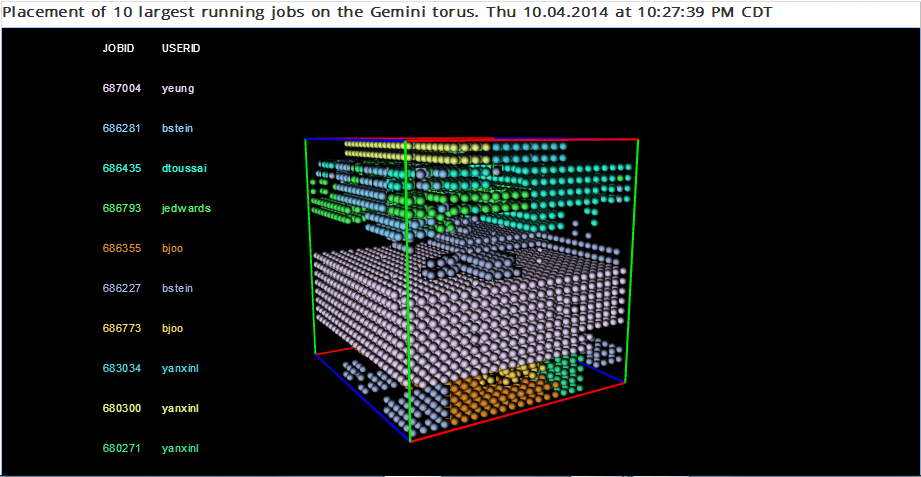
\includegraphics[width=3.0in]{capture}
	\caption{
        System utilization view showing the node placements for the ten largest
        jobs running on the Blue Waters system.  Users and other stakeholders
        are given a live, birds-eye-view of the system, that depict such
        features as overall utilization, relative job sizes, and placement
        fragmentation.
    }
	\label{tv1}
\end{figure}

    As another use case, the location of the largest running jobs can be
    shown by visualization tools as an indication of the system utilization. A
    portal plugin has been developed for this purpose. Figure ~\ref{tv1} shows a
    screen shot of the Blue Waters portal system status page. The page shows,
    among other things, the location and identification of the ten largest jobs
    on the system at the time the page was loaded. Refreshing the page reloads
    new information. The node placements are color coded by job. User
    information is also provided and colored to match their particular job's
    nodes. The arrangement of nodes is surrounded by a bounding box. The color
    of the box edges indicates the direction of the torus. Red edges run in the
    X direction, green edges in the Y direction, and blue edges in the Z
    direction. One can see the bias in job distribution away from the Y
    direction. This direction has less communication performance than the other
    directions. 

    In order to understand the utility of the system, we describe briefly the
    data collection and display mechanisms used, here.  In the context of this
    work, the data collection is done by mining system logs and placing the data
    in a database. In particular, the job scheduler system logs contain
    information about when jobs start and end as well as what nodes are used.
    This dynamic information is read and stored at regular intervals.  Other
    static information such as the location of compute nodes on the
    communication fabric and the location of service nodes in the fabric is also
    stored in the database.  Delivery of this representation to a geographically
    distributed user base can be most easily accomplished via a web based
    interface, so the viewer extracts near real-time data and displays the
    information on a web browser.

%%%%%%%%%%%%%%%%%%%%%%%%%%%%%%%%%%%%%%%%%%%%%%%%%%%%%%%%%%%%%%%%%%%%%%%%%%%%%%%
% ARCHITECTURE %%%%%%%%%%%%%%%%%%%%%%%%%%%%%%%%%%%%%%%%%%%%%%%%%%%%%%%%%%%%%%%%
%%%%%%%%%%%%%%%%%%%%%%%%%%%%%%%%%%%%%%%%%%%%%%%%%%%%%%%%%%%%%%%%%%%%%%%%%%%%%%%

\section{Architecture}
    Due to its broad applicability, many desirable features or capabilities were
    suggested during our early design and prototyping efforts.  We began to
    notice a number of recurring requirements that many of our use cases shared
    in common.  For TorusVis, we identified these requirements, and set out to
    meet them as our primary design goals.

    \subsection{Requirements}
        Our highest priority goal was to design TorusVis to be generic, and
        applicable to as many topology data presentation scenarios as possible.
        During our initial study on application run time consistency, we had
        many small codes that would produce some form of visualization of the
        Blue Waters torus topology.  Each would do so in a different way, and
        emphasize certain features or attributes that serve slightly different
        purposes.  They were created for a specific use and often required
        significant, involved changes when new needs were identified.  We also
        learned that some of our industry collaborators were working on their
        own similar set of torus visualization tools, and noted that between us,
        there were at least half a dozen different in-house tools producing
        slightly different visualizations of what was essentially the same
        subject.  We set out to create a software library that could replace
        most of the functionality of these disparate applications with a single
        general-purpose code base.
    
        To promote this broad applicability, we designed TorusVis to be
        extensible and flexible.  For every major step of the topology
        visualization process, the default behavior can be extended or
        completely replaced with application-specific logic.  Our design
        identifies three of these features and formulates the process as a data
        flow between layers, one for each step (section
        \ref{subsection_design}).  Each layer provides a set of commonly used
        data structures and routines and serve as extension points for
        applications.  This flexibility allows many users to adapt TorusVis to
        their specific needs while also taking advantage of the core
        visualization functionality needed for most applications.  

        Finally, despite being extensible and generic, we try to keep TorusVis
        simple where practical.  We target a user audience that primarily
        consists of domain experts and administrators; users that may not be
        willing or able to devote time to learning the details of a complex
        software design.  Furthermore, we expect that some applications and
        visualizations produced will target project stakeholders or a more
        public audience, such as in the case where they are used as a
        dissemination tool.  TorusVis must be simple in design to promote
        improvements throughout development, expose a simple API that is readily
        extensible for applications, and facilitate applications with wide
        accessibility.  Wherever possible, the barrier to entry for development,
        application, and presentation is kept to a minimum.

    \subsection{Features}

        TorusVis is a software library for web applications in JavaScript and
        accessible over a web browser.  We note that JavaScript enjoys a
        simplified object model that lends itself well to developing flexible
        asynchronous applications and promotes fast turn-around time for the
        write-deploy-test cycle typical of most agile development styles.
        TorusVis uses the 3D graphics library, three.js\cite{threejs}, which
        enables rendering with native graphics hardware for browsers that
        support it (see: WebGL\cite{webgl}).  It is entirely front-end code,
        leaving the task of accessing data from back-end stores to applications.

    \subsection{Design}
        \label{subsection_design}

        \begin{figure}[!t]
            \centering
            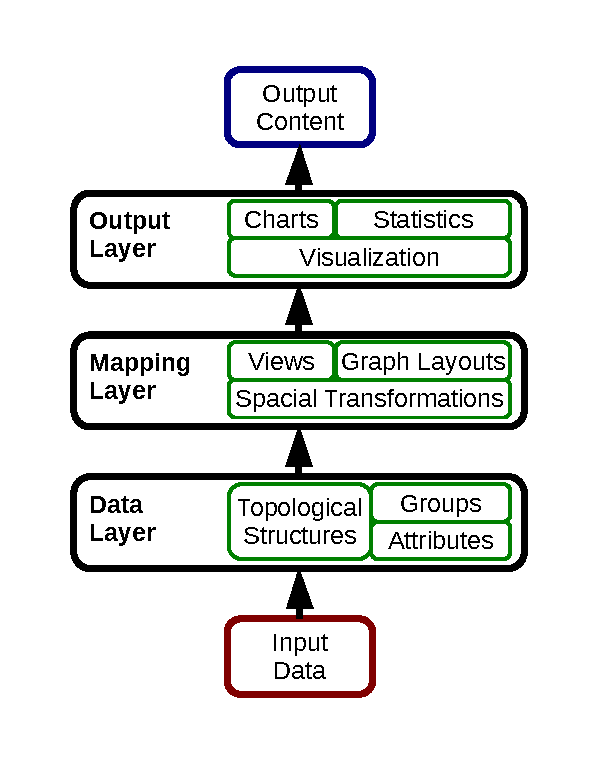
\includegraphics[width=2.5in]{design-diagram}
            \caption{Diagram depicting the overall design of TorusVis.}
            \label{fig_design}
        \end{figure}

        The design of TorusVis is centered around a set of high-level steps
        we've identified as common to most topology data visualization
        applications.  The API is logically split into three major layers, each
        corresponding to step in the visualization process (Figure
        \ref{fig_design}).  The steps can be described as 1 -- collecting data
        in generic structures, 2 -- mapping these data structures to concrete
        forms, and 3 -- reducing the data into a visualization.  We've found
        that this workflow matches well with a large range of applications,
        provides ample opportunity for domain-specific extensions, and is simple
        to understand.

        The data layer is the first and is concerned with providing graph data
        structures and high-level visualization primitives.  Here, the nodes and
        edges of the system topology are defined.  Additional arbitrary data can
        be associated with nodes or edges as attributes.  For visualization, one
        or more sets of nodes or edges are also defined in the form of groups.
        Groups are selections of a subset of a graph's nodes or edges that are
        to be rendered, and are also associated with a set of options that
        control the visual characteristics at a high level, such as color, size,
        and shape.  Groups can be used to represent the set of nodes in a job's
        allocation, a set of links along a path of interest, or any set of
        components that match a criteria.
 
        \begin{figure*}[!t]
            \centering
            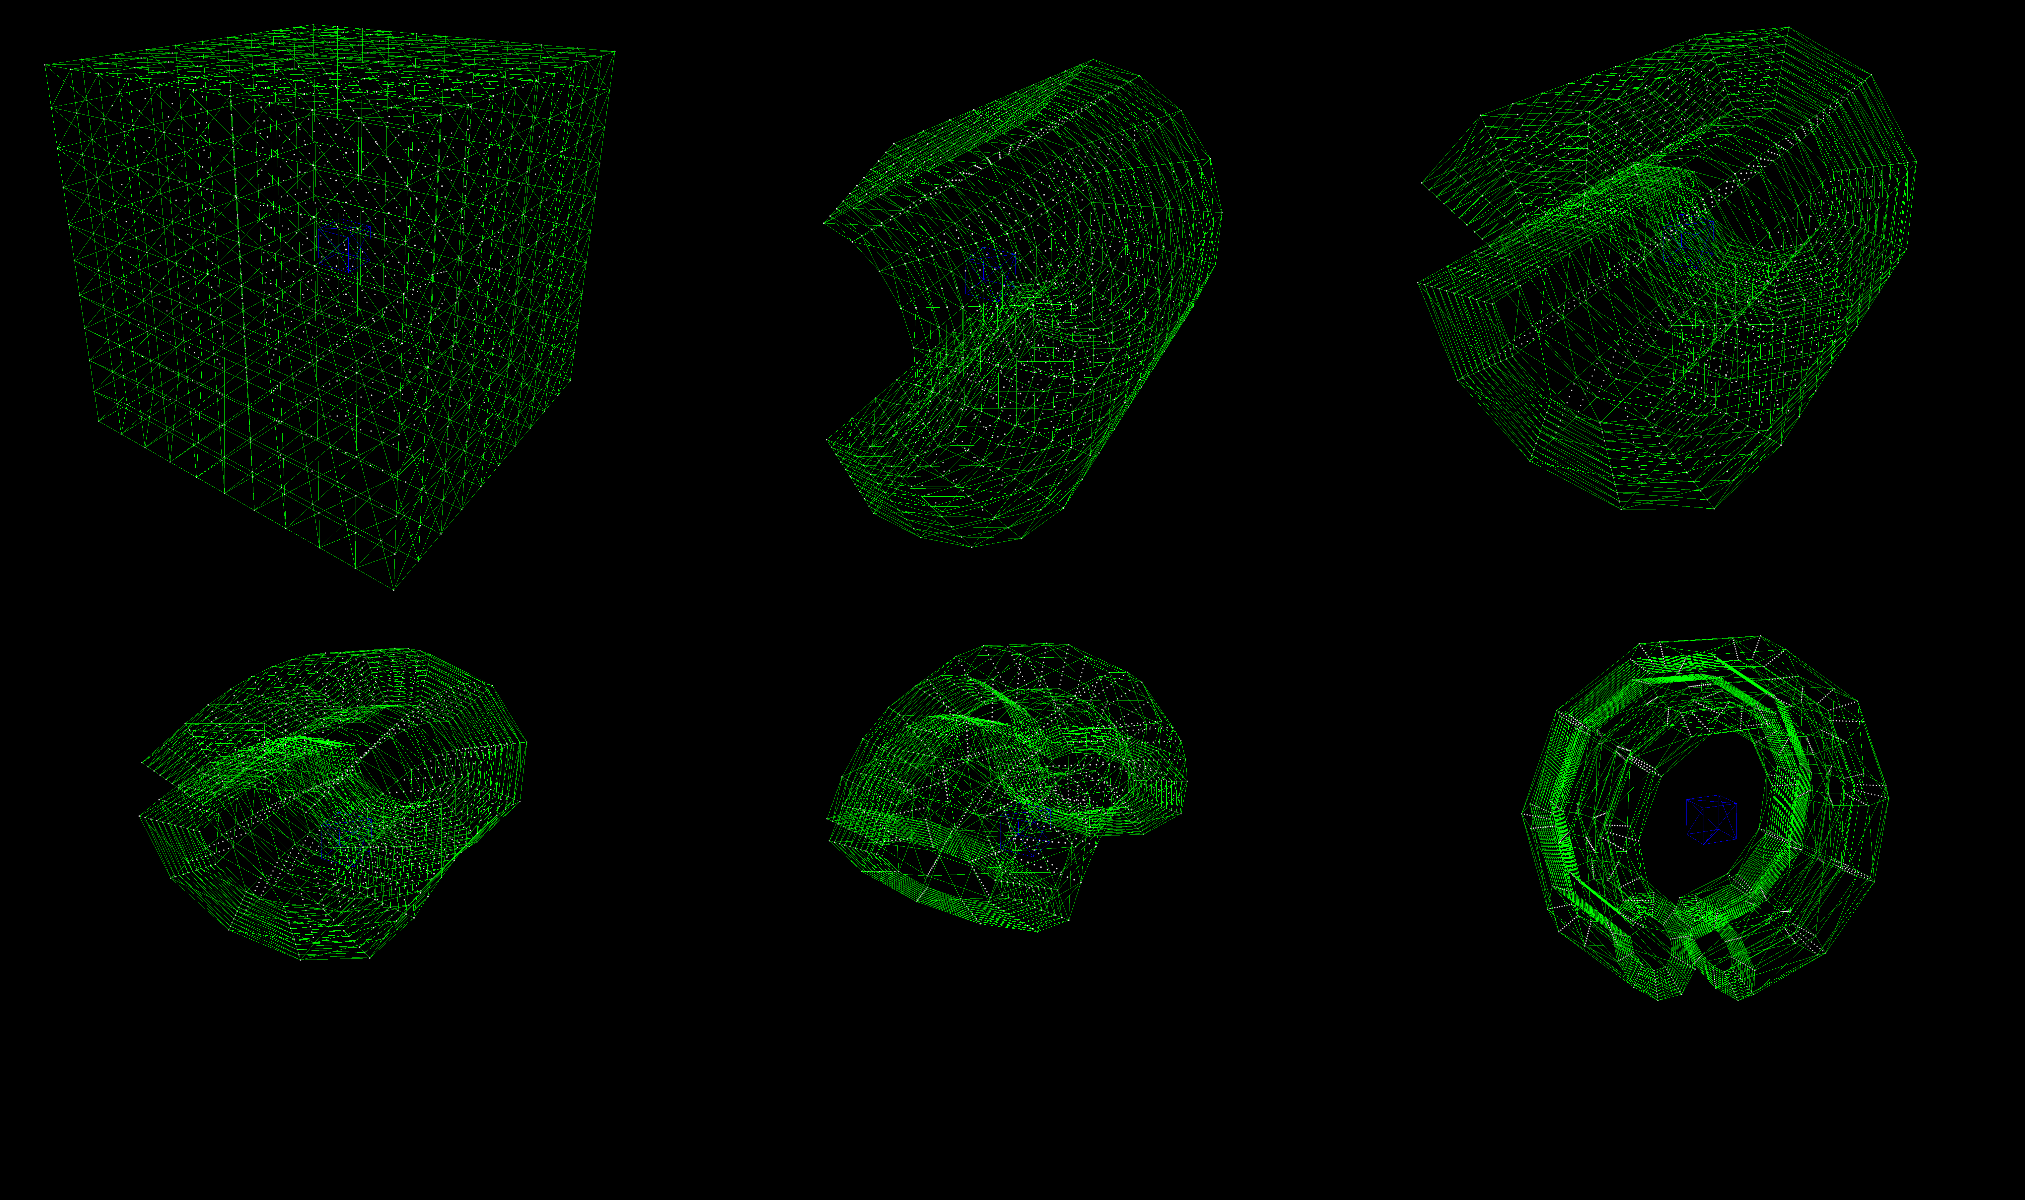
\includegraphics[width=6.5in]{torus}
            \caption{
                Example application demonstrating an alternative mapping
                implementation.  Here, the spacial embedding of a square torus
                is wrapped radially along two dimensions (\emph{top and
                bottom}), with each view showing the progression of the
                transformation (\emph{left to right}).
                }
            \label{fig_torus}
        \end{figure*}
  
        The mapping layer provides the tools to transform abstract topology data
        collected in the data layer to a concrete form more suitable for
        visualization.  It is primarily concerned with defining an embedding of
        the given topology that associates each node with a point in 3D space,
        and each edge with a set of such points along which a path may be drawn.
        For example, a simple mapper might just query the attributes of each
        node, or another might apply an automatic graph layout algorithm.  Other
        examples include mappers that provide different ``views'' of the same
        data, or mappers that apply spacial transformations, such as cycling the
        nodes of a torus topology along a periodic dimension, or wrapping a
        cartesian embedding into one in a polar space to reinforce the
        periodicity (Figure \ref{fig_torus}).

        The output layer provides the visualization capabilities.  An instance
        of the output layer encapsulates a specific routine that produces a
        rendering from the information in the first two layers.  Recall that the
        layers can be extended, and therefore can be made to exhibit
        application-specific behavior that might not match with their intended
        use.  This possibility is especially relevant for the output layer,
        where implementations are at liberty to produce any manner of
        visualization, or even content that are not visualizations, at all.
        While not the intended use, there are no restrictions in our design of
        TorusVis that would prevent output layer implementations from creating
        other charts, tables of summary statistics, or audio clips if client
        applications were so inclined.

%%%%%%%%%%%%%%%%%%%%%%%%%%%%%%%%%%%%%%%%%%%%%%%%%%%%%%%%%%%%%%%%%%%%%%%%%%%%%%%
% DISCUSSION %%%%%%%%%%%%%%%%%%%%%%%%%%%%%%%%%%%%%%%%%%%%%%%%%%%%%%%%%%%%%%%%%%
%%%%%%%%%%%%%%%%%%%%%%%%%%%%%%%%%%%%%%%%%%%%%%%%%%%%%%%%%%%%%%%%%%%%%%%%%%%%%%%

\section{Discussion}

    Analysis and visualization of system data offer essential guidance in
    maximizing the productive value of HPC resources.  The growing scale of
    modern systems have placed greater emphasis on topological considerations
    that require new methods and tools to better understand.  We described our
    early topology visualization applications, initially created for our study
    of application run time consistency, and demonstrate their value in a number
    of use case studies.  As more small and disparate visualization applications
    were created for various purposes, the value in a general purpose tool
    became apparent. We channeled the development experiences gained while
    creating our early prototypes into a software library we call ``TorusVis''.
    We discuss the design of TorusVis, and how it meets our requirements for
    generality, flexibility, and simplicity.

    The design of TorusVis allows applications to replace or supplement most
    provided functionality with application- or domain-specific behavior.  This
    flexibility has great potential to support a broad range of use cases as
    well as provide a platform for future research and development.  For
    example, we found that characterizing the relationship between job node
    placement and application performance through rigorous, quantitative
    assessment is exceptionally difficult and highly application-specific in
    nature.  TorusVis applications can help users prepare and run their jobs in
    ways more topologically-aware, by offering them an intuitive and qualitative
    sense of this relationship, leading to better informed preferences for node
    sets, allocation shapes, and other system features.  Submitting
    computational workloads in more topology-sensitive configurations might
    decrease average job turnaround time, increase overall utilization, and
    reduce the risk and impact of failures.

    TorusVis is still very young in its development.  Our future plans are to
    complete a modest number of features still missing from our early prototypes
    and release the library under an open-source license.  The potential in
    having a tool that supports such a large class of HPC systems operations
    tasks developed over a collaborative, open access medium should not be
    understated.  We feel the HPC community have only recently begun to
    seriously contend with topology issues, and applying combined and focused
    efforts that benefit all stakeholders should be preferred over individual
    disparate developments.  We hope to promote our own efforts, but also engage
    the broader community -- to initiate an open dialogue on topology issues
    and collective efforts towards unified solutions.

    We hope to further explore possibilities in topology visualization research
    by applying TorusVis to other networking technologies and system topologies,
    such as the Gordon system at the San Diego Supercomputer Center, an
    infiniband torus network, future systems using Cray's "Dragonfly"
    technology, and also smaller-scale fat tree topologies.
%%%%%%%%%%%%%%%%%%%%%%%%%%%%%%%%%%%%%%%%%%%%%%%%%%%%%%%%%%%%%%%%%%%%%%%%%%%%%%%


%%%%%%%%%%%%%%%%%%%%%%%%%%%%%%%%%%%%%%%%%%%%%%%%%%%%%%%%%%%%%%%%%%%%%%%%%%%%%%%
% PRIOR WORK %%%%%%%%%%%%%%%%%%%%%%%%%%%%%%%%%%%%%%%%%%%%%%%%%%%%%%%%%%%%%%%%%%
%%%%%%%%%%%%%%%%%%%%%%%%%%%%%%%%%%%%%%%%%%%%%%%%%%%%%%%%%%%%%%%%%%%%%%%%%%%%%%%

\section{Prior Work}
    Collections of system monitoring data often hold key insights that inform
    efforts to operate HPC resources as well as optimally exploit them for
    domain applications \cite{Brandt:2009}.  For example, fine-grained data at
    the component level can help maintenance staff identify and correct
    failures; and users to determine optimization strategies that are most
    promising.  As the scale of HPC systems increase and the number of their
    components continue to grow, the respective increase in system data have
    necessitated new methods and tools to analyze
    \cite{Lee:2008,Muelder:2009,Schulz:2011}.  Visualizing analysis results in
    multiple contexts or domains has been shown to more clearly highlight their
    important features \cite{Schulz:2011,Bhatia:2005}.  In particular,
    understanding network traffic patterns is of great importance for many
    applications, and visualizing these patterns on multiple 2D and 3D views
    that resemble the topology of the system interconnect provides insight
    valuable to both application developers and performance engineers
    \cite{Landge:2012}.

    Our current development focuses on working with directed graph structures, a
    representation we expect would be general enough to be adapted to most
    topology data sets.  We also note that visualizations of similar data, but
    in less generic forms (Gantt charts, timeline views, scatter plots, etc.) are
    already extensively covered by existing methods and tools
    \cite{Herrarte:1991,Heath:1991,Heath:1994,Karrels:1994,Kranzlmuller:1996,
    Nagel:1996,Jerding:1997,Kranzlmuller:1998,Topol:1998,Shaffer:1999,
    Wu:2000,Shende:2006,Chan:2007,Moreta:2007,Cornelissen:2008}.  Prior software
    systems for analyzing graph data have typically combined graph layout
    algorithms and visualization features
    \cite{Ellson:2001,Bastian:2009,Moscovich:2009,Auber:2010,
    Pinaud:2012,Zaidi:2012}.  We chose not to focus on graph layout features
    since in the most common use cases, users will already have one of possibly
    several layouts predetermined, such as that of the interconnect topology,
    one depicting the virtual topology of an application, or a physical map of
    where the system hardware components lie in a data center.  Despite this
    omission, we suspect that automatic graph layout capabilities will
    eventually prove to be a worthwhile addition and another avenue for future
    research and development.

%%%%%%%%%%%%%%%%%%%%%%%%%%%%%%%%%%%%%%%%%%%%%%%%%%%%%%%%%%%%%%%%%%%%%%%%%%%%%%%
% ACKNOWLEDGEMENT %%%%%%%%%%%%%%%%%%%%%%%%%%%%%%%%%%%%%%%%%%%%%%%%%%%%%%%%%%%%%
%%%%%%%%%%%%%%%%%%%%%%%%%%%%%%%%%%%%%%%%%%%%%%%%%%%%%%%%%%%%%%%%%%%%%%%%%%%%%%%

\section*{Acknowledgment}

    We would like to thank our collaborators at Cray and Adaptive Computing for
    their help in the application run time consistency testing that served as
    the initial motivation for this project.  We would also like to thank our
    colleagues Celso Mendes, Robert Sisneros, Galen Arnold, and Greg Bauer for
    their valuable contributions and feedback.

    This research is part of the Blue Waters sustained-petascale computing
    project, which is supported by the National Science Foundation (award number
    ACI 1238993) and the state of Illinois. Blue Waters is a joint effort of the
    University of Illinois at Urbana-Champaign and its National Center for
    Supercomputing Applications.

%%%%%%%%%%%%%%%%%%%%%%%%%%%%%%%%%%%%%%%%%%%%%%%%%%%%%%%%%%%%%%%%%%%%%%%%%%%%%%%
% REFERENCES %%%%%%%%%%%%%%%%%%%%%%%%%%%%%%%%%%%%%%%%%%%%%%%%%%%%%%%%%%%%%%%%%%
%%%%%%%%%%%%%%%%%%%%%%%%%%%%%%%%%%%%%%%%%%%%%%%%%%%%%%%%%%%%%%%%%%%%%%%%%%%%%%%

% \IEEEtriggeratref{26}
% \IEEEtriggercmd{\enlargethispage{-5in}}

\bibliographystyle{IEEEtran}
\bibliography{references}

\end{document}

